% --------------------------------------------------------------------------- %
% --------------------------------------------------------------------------- %
\chapter{The LHC and The CMS Experiment}
\label {ch:cms}

\section{The Large Hadron Collider}
The Large Hadron Collider (LHC) is the largest particle accelerator in the world~\cite{lhcmachine}.
It is designed to collide protons against other protons with a center of mass energy up to 14 TeV.
The first collisions used for physics happened in March 2010, when the LHC was running at a center of mass energy of 7 TeV.
The LHC was restarted the following year and operated at a higher energy of 8 TeV
eventually delivering about four times the amount of data that was taken at 7 TeV.
After the successful first run ended, the machine was shut down in order to upgrade many components.
The next time the LHC was run was in May 2015, where protons were successfully collided at a center of mass energy of 13 TeV.
The analysis shown in this thesis is based on the data taken during the 2015 running period at 13 TeV.

In order to achieve such large center of mass energies,
the protons are accelerated in two separate circular beam pipes which are 27 km long and and 100 m underground.
These beam pipes are kept as close as possible to vacuum in order to minimize the interaction of protons with other particles.
Since the pipe is circular,
it's possible to accelerate two beams of protons in opposite directions and repeatedly collide them at various points around the ring.
There are 4 points along the ring where protons are made to collide and the resulting collisions are recorded by various experiments as seen in figure~\ref{fig:lhcunderground}.
The Compact Muon Solenoid (CMS) experiment~\cite{jinst} is where the data was taken used for the results shown in this thesis.

\begin{figure}[!ht]
  \begin{center}
    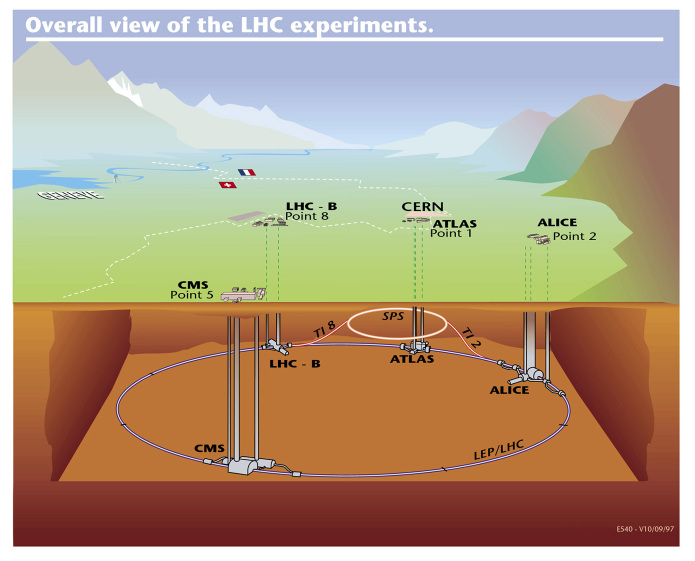
\includegraphics[width=0.8\textwidth]{cms/figs/lhc-underground.jpeg}
    \caption{ The LHC can be seen along with the 4 main experiments at different points along the beamline.
      \label{fig:lhcunderground}
    }
  \end{center}
\end{figure}

\section{Physics Processes and Cross Sections}
Particle physics processes are studied by measuring various quantities such as particle masses,
lifetimes, and production rates both inclusively and differentially with respect to certain kinematic variables.
When protons collide,
it is not the protons themselves that interact but rather the constituents, or partons, that make up the proton.
The formula describing this is given in equation~\ref{eqn:nevts}.
The number of events expected for a specific physics process is given by three quantities.
The integrated luminosity ($\mathcal{L}$) is dependent on the brightness of the proton beam.
The cross section for the event to happen ($\sigma$),
which includes the branching fraction for a particle to decay to a specific final state,
is a fundamental physics quantity.
the units for cross section is ``barns'', and a barn is defined as $\mathrm{10^{-24}~cm^{2}}$.
Lastly, the efficiency for the event to be reconstructed ($\epsilon$) is completely determined by the detector.

\begin{equation}
\label{eqn:nevts}
  \mathrm{N_{events} = \mathcal{L} * \sigma * \epsilon}
\end{equation}

Protons can interact elastically (scattering) or inelastically, meaning they are destroyed in the process.
The inelastic cross section for two protons to collide at a center of mass energy of 13 TeV is about 100 mb.
This can be seen in figure~\ref{fig:xsecs} along with the cross section values for other interesting
standard model processes.
Other processes that are main backgrounds in the signal region of this analysis are Drell-Yan and $\mathrm{t\bar{t}}$ production
which have a cross section at 13 TeV of roughly 4 nb, and 0.8 nb respectively.
Taking into account all the branching fractions and detector efficiencies,
these processes are reconstructed roughly once in a billion (trillion) times per inelastic proton collision for Z ($\mathrm{t\bar{t}}$) production.

\begin{figure}[!ht]
  \begin{center}
    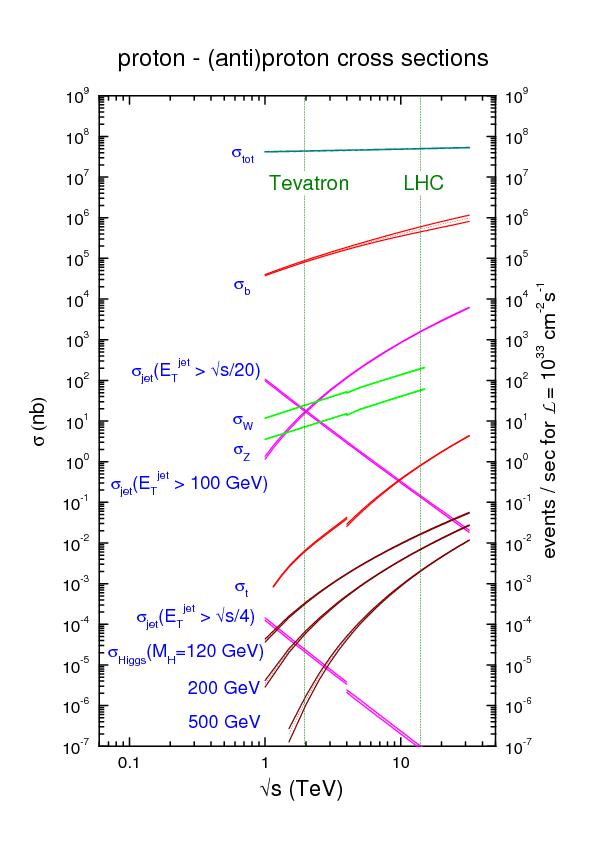
\includegraphics[width=0.8\textwidth]{cms/figs/cross-sections.png}
    \caption{
      The cross section values for various standard model processes is shown in this figure as a
      function of the center of mass energy of two protons colliding.
      \label{fig:xsecs}
    }
  \end{center}
\end{figure}

The peak instantaneous luminosity measured in a given day during the 2015 data taking period is shown on the left in figure~\ref{fig:peaklumi},
and the highest value is 5.13 $\mathrm{\frac{Hz}{nb}}$.
This means that approximately $\mathrm{10^{8}}$ protons collide per second.
The rate of collisions is much larger than the capacity for the detector to write out data,
and as discussed previously, most of these events are just soft inelastic collisions of two protons.
In order to maximize the efficiency of collecting data that is useful to any physics analysis,
a triggering system is put in place which only writes out the event information if certain conditions are met.
The maximum rate of all the concurrent triggers in CMS is about 1 kHz.
The total luminosity collected in 2015 was 3.81 $\mathrm{fb^{-1}}$ which can be seen on the right in figure~\ref{fig:peaklumi},
but due to data quality issues the amount that was useable for physics analysis was 2.26 $\mathrm{fb^{-1}}$.

\begin{figure}[!ht]
  \begin{center}
    \begin{tabular}{c c}
      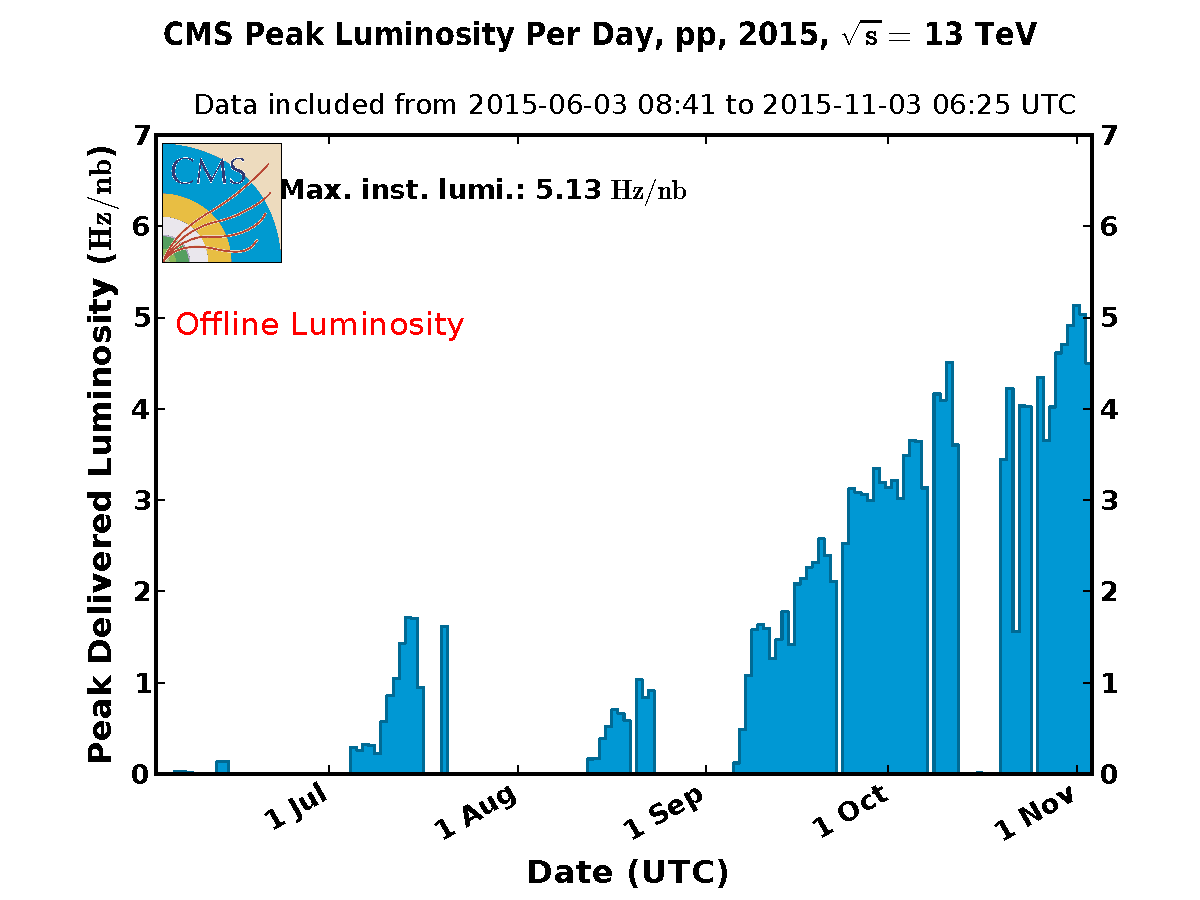
\includegraphics[width=0.4\textwidth]{cms/figs/peak_lumi_per_day_pp_2015.pdf} &
      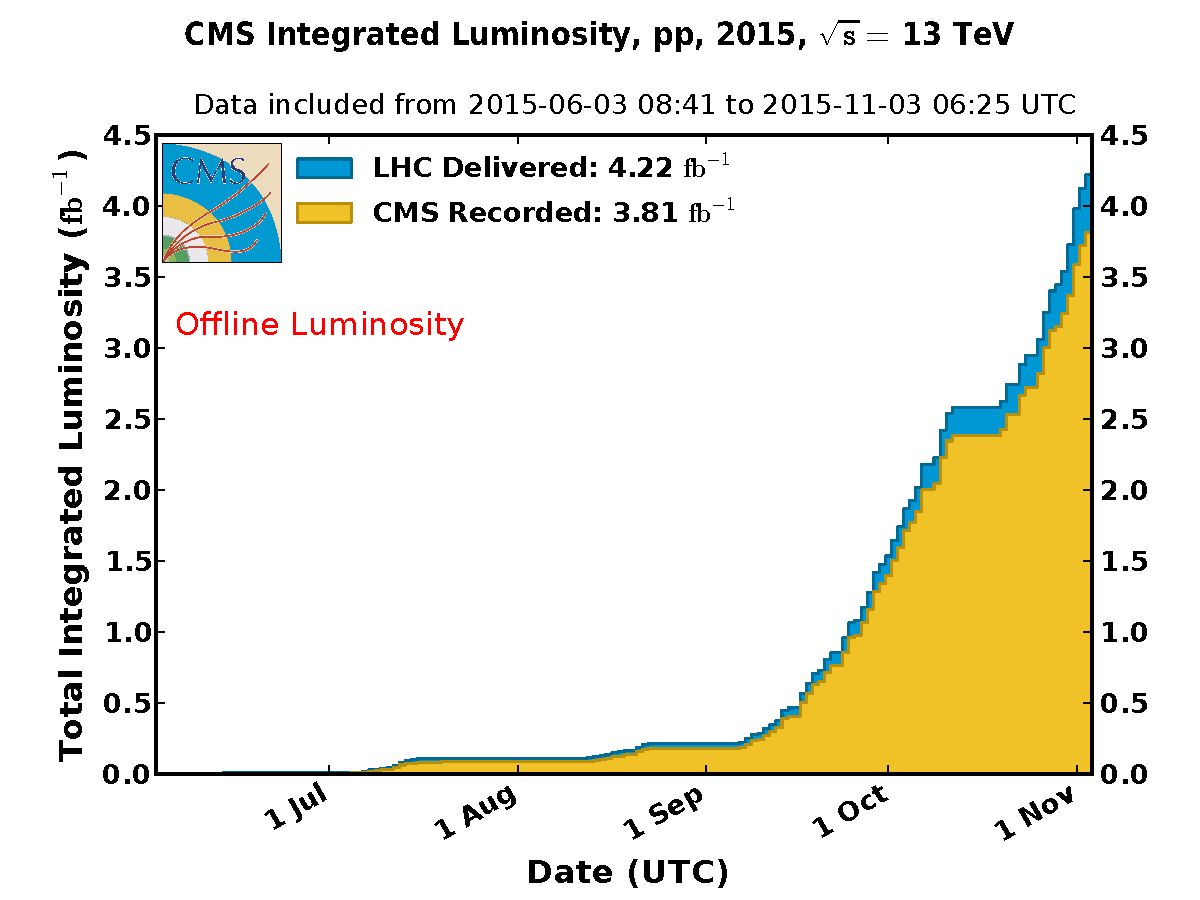
\includegraphics[width=0.4\textwidth]{cms/figs/int_lumi_per_day_cumulative_pp_2015.pdf} \\      
    \end{tabular}
    \caption{
      The peak instantaneous luminosity per day during the 2015 data taking period is shown on the left
      and the total integrated luminosity is shown on the right in this figure.
      \label{fig:peaklumi}
    }
  \end{center}
\end{figure}

\section{Particle Interactions With Matter}

The total amount of energy lost by a particle when interacting with matter is mainly due to two effects,
interactions that lead to the particle decaying or ``showering'',
and energy loss by ionization.
Two equations are used to describe energy loss due to showering,
equations~\ref{eqn:radiation_length} describes particle interactions via QED processes,
and~\ref{eqn:interaction_length} describes particle interactions via QCD processes.
Equation~\ref{eqn:radiation_length} represents the average energy left over as a particle travels a distance x through a material with radiation length ($X_{0}$).
Equation~\ref{eqn:interaction_length} represents the average number of particles left when $N_{0}$ particles traverse a distance x through a material with interaction length ($\lambda_{int}$).
The largest source of uncertainty when measuring a particle's energy using the ECAL or HCAL is called the ``stochastic term''
and is mostly due to intrinsic statistical shower fluctuations and sampling fluctuations.
The energy of a parton is distributed evenly among all of its decay products on average,
so the initial particles energy is proportional to the number of decay products $E_{0} \propto N_{0}$.
The overall uncertainty due to the stochastic term becomes proportional to $\sqrt{N_{0}}$ in the limit where N is large.

\begin{equation}
  \label{eqn:radiation_length}
  E(x) = E_{0}e^{\frac{-x}{X_{0}}}  
\end{equation}

\begin{equation}
  \label{eqn:interaction_length}
  N(x) = N_{0}e^{\frac{-x}{\lambda_{int}}}  
\end{equation}

Typical values for radiation and interaction lengths are shown in table~\ref{tab:rad_int_lengths}
for the different materials making up the tracker (silicon), ECAL (PbWO4) and HCAL (Copper).
In table~\ref{tab:materialbudget}, the depth of each of these materials corresponding to $|\eta| = 0$ is shown as a function of $X_{0}$ and $\lambda_{int}$.
The values in tables~\ref{tab:rad_int_lengths}~and~\ref{tab:materialbudget} are taken from a talk given at CERN in May 2016~\cite{calorimetry}.
Based on these values, an electron or photon loses at least \textasciitilde{}40\%
of its energy on average when traveling through the tracker before it is incident on the ECAL.
This means either has a relatively high chance of interacting, where a photon might pair-produce and an electron might brem a photon.
These effects are taken into consideration when reconstructing photons and electrons and better-described in chapter~\ref{ch:evtsel}.

Another effect that can be seen is in the HCAL, which is a ``sampling'' calorimeter.
A sampling calorimeter is designed to have layers of material with large
$\lambda_{int}$~interpsered with layers of material that are used to measure particles.
This is described in more detail in subsection~\ref{subs:HCAL}.
In the HCAL in CMS, there are 16 layers of absorber material.
This means that each layer has more than 4.5 radiation lengths.
When a hadronic shower evolves, approximately 30\% of the shower is in the form of EM energy.
4.5$\mathrm{X_{0}}$ is essentially deep enough to completely contain the EM component of the hadronic shower before it can be measured.
This leads to an increased uncertainty of the initial parton's energy.

\begin{table}[htb]                                                                                                                                                              
  \begin{center}
    \caption{
      \label{tab:rad_int_lengths}
      Radiation ($\mathrm{X_{0}}$) and interaction lengths ($\lambda_{int}$) for various materials that make up different sub-detectors in CMS.
    }
    \begin{tabular}{l|c|c}
      \hline
      \hline
      Material & $\mathrm{X_{0}}$ [cm] & $\lambda_{int}$ [cm] \\
      \hline
      Silicon                             & 9.36 & 45.5 \\
      Lead Tungstate (PbW$\mathrm{O_{4}}$) & 0.88 & 19.5 \\
      Copper                              & 1.43 & 15.1 \\
      \hline
      \hline
    \end{tabular}
  \end{center}
\end{table}

\begin{table}[htb]                                                                                                                                                              
  \begin{center}
    \caption{
      \label{tab:materialbudget}
      Material budget of tracker and calorimeters in CMS at $|\eta|=0$ as a function of radiation ($\mathrm{X_{0}}$) and interaction ($\lambda_{int}$) lengths.
    }
    \begin{tabular}{l|c|c}
      \hline
      \hline
      Material & Radiation lengths [$\mathrm{X_{0}}$] & Interaction lengths [$\lambda_{int}$]  \\
      \hline
      Silicon                             & 0.5 & 0.1 \\
      Lead Tungstate (PbW$\mathrm{O_{4}}$) & 25 & 1.1 \\
      Copper                              & 73.9 & 7 \\
      \hline
      \hline
    \end{tabular}
  \end{center}
\end{table}

Energy loss by ionization is mostly due to a particle having elastic collisions with electrons and can be characterized by the Bethe-Bloch formula shown in equation~\ref{eqn:bethebloch}.
In this equation, K is a constant equalling 0.307 MeV $\mathrm{g^{-1}}cm^{2}$,
$\mathrm{T_{max}}$ is the max energy transfer in a single collision,
$z$ is the charge of the incident particle,
Z is the charge number of the medium,
A is is the atomic mass of the medium,
$m_{e}$ is the mass of an electron,
and I is the mean excitation energy of the medium.
Muons have a low interaction cross section with the materials used to build CMS in the energy range that they are produced when coming from Z bosons produced at the LHC.
They are referred to as minimum ionizing particles, and the stopping power of copper on muons can be seen in figure~\ref{fig:muonenergyloss}.
Therefore, muons do not deposit very much energy in any of the calorimeters.
Typical momenta of muons in this analysis are between 20-200 GeV.
When muons have momenta greater than 200 GeV, radiative losses start to become the primary reason for energy loss.

\begin{equation}
  \label{eqn:bethebloch}
-<\frac{dE}{dx}> = Kz^{2}\frac{Z}{A}\frac{1}{\beta^{2}}[\frac{1}{2}ln\frac{2m_{e}c^{2}\beta^{2}\gamma^{2}T_{max}}{I^{2}}-\beta^{2}-\frac{\delta(\beta\gamma)}{2}]
\end{equation}

\begin{figure}[!htb]
  \begin{center}
    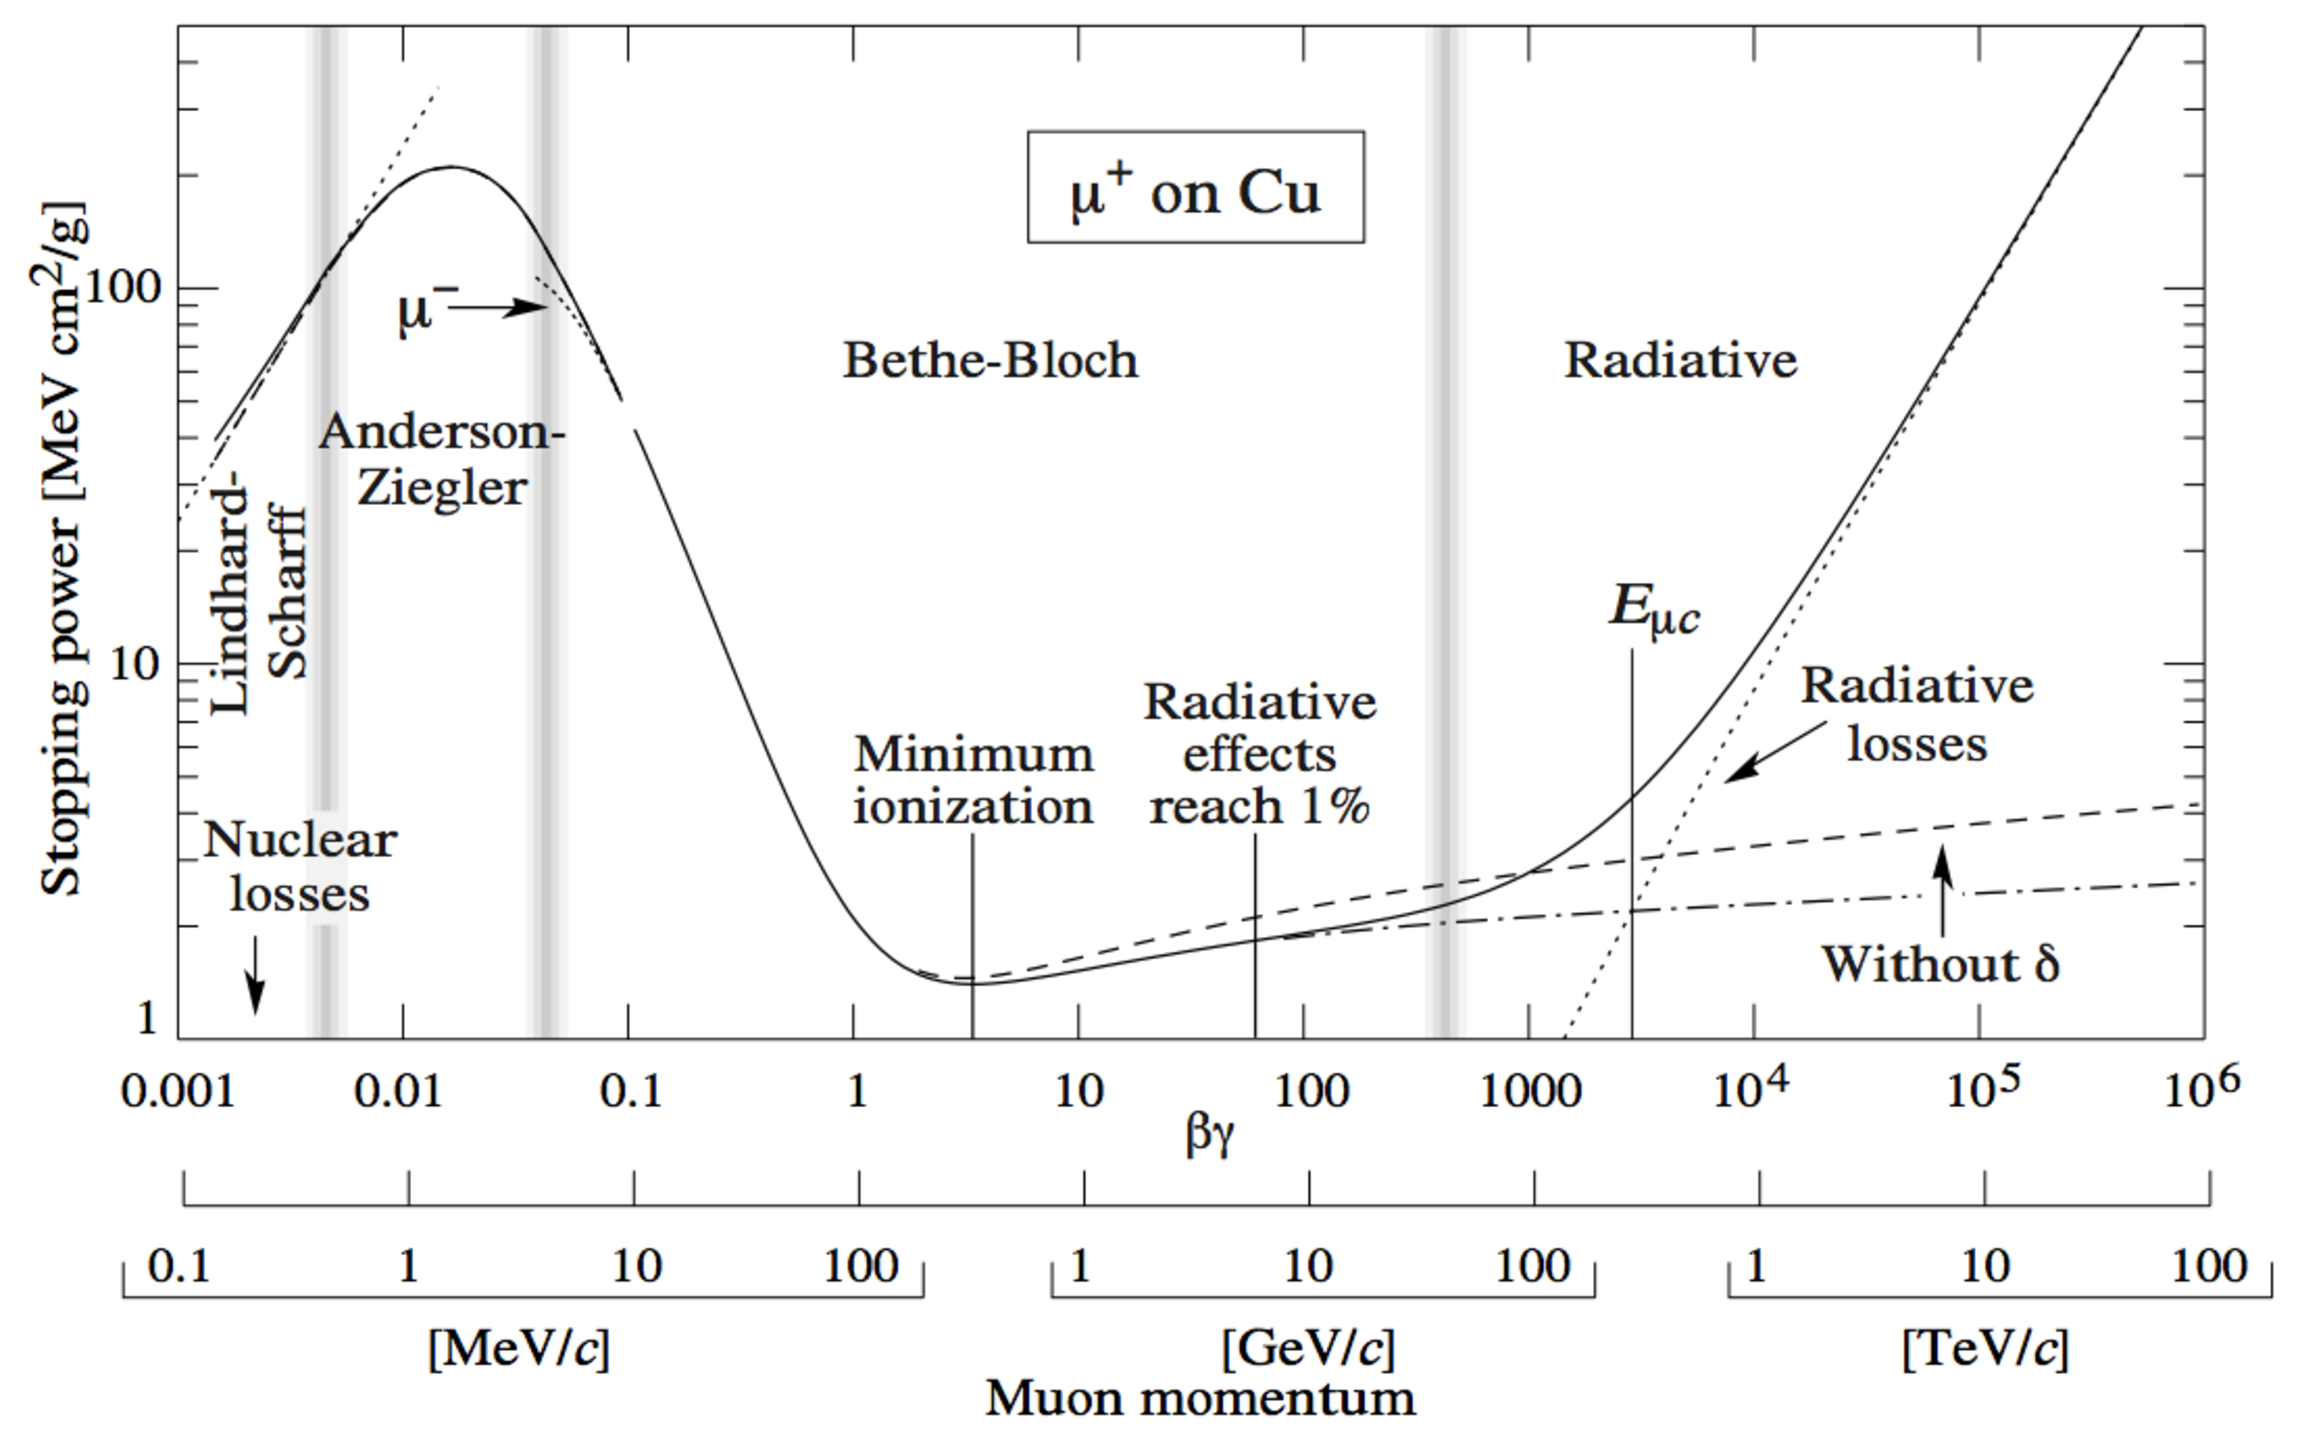
\includegraphics[width=0.8\textwidth]{cms/figs/muon_energy_loss.pdf}
    \caption{
      \label{fig:muonenergyloss}
      Stopping power of copper as a function of muon momentum. Typical momenta of muons in this analysis are between 20-200 GeV.
    }
  \end{center}
\end{figure}

\section{The Compact Muon Solenoid}
The CMS detector consists of a triggering system and many sub detectors,
where measurements taken using these sub detectors are used as input to the triggering system.
When protons are collided at the interaction point within CMS, approximately N collisions happen per second.
The rate of collisions is so high that it is impossible to record all of the data all of the time.
The way this is controlled is by the use of triggers, the level 1 (L1) trigger and the high level triggers (HLT).
The triggers are designed such that the full event information is stored when all the requirements of a trigger are met.
For some physics processes, trigger rates are much higher than can be afforded by the allowed budget of the CMS experiment.
These processes can still be studied by prescaling the triggers meaning the full information is saved once per N events.
As the prescale N is increased, the rate of the trigger is reduced.

The CMS sub detector components are layered in such a way that one can take advantage of different particle interactions with different materials.
The innermost layer is the tracker (decribed in section~\ref{subs:tracker}) which is used to measure the charge and momentum of charged particles.
When a charged particle passes through the silicon tracker's layers, a small amount of energy is deposited.
The deposit is large enough that a hit will be registered by the electronics, but small enough that the trajectory of the particle will be minimally affected.

The next layer is the Electromagnetic Calorimeter (decribed in section~\ref{subs:ECAL}) which is used to contain and measure the energy of electrons and photons.
The Electromagnetic Calorimeter (ECAL) is made of lead tungstate ($\mathrm{PbWO_{4}}$) scintilating crystals.
Electrons and photons that enter the ECAL lose energy due to showering, and the depth of the ECAL is sufficient enought to fully contain these particles.

Outside of the ECAL is the Hadronic Calorimeter (decribed in section~\ref{subs:HCAL}) which is used to contain and measure the energy of hadronic particles.
The Hadronic Calorimeter (HCAL) is designed in such a way that hadronic particles incident on the HCAL lose energy to showering.
The goal is to fully contain these particles, although sometimes particles have sufficient energy that they are able to escape before losing sufficient energy to showering.
This phenomenon is known as punch-through.

Beyond the HCAL is the solenoid which produces a magnetic field of 3.8 T at the center of the detector.
This magnetic field is used to bend the tracks of charged particles in order to measure the momentum following the equation~\ref{eqn:bfieldmomentum},
where q is the particle charge, r is the radius of curvature, and B is the magnetic field magnitude.

\begin{equation}
  \label{eqn:bfieldmomentum}
p = qrB
\end{equation}

The only particles that should pass beyond the HCAL are muons and neutrinos.
Neutrinos are measured indirectly by assuming that the momentum in the direction transverse to the beam is zero at the beginning of each collision,
and then calculating the sum of the total transverse momentum of all particles directly measuered in the detector.
Since Neutrinos pass through the detector with no interactions, they contribute to missing transverse momentum, which will be referred to as (\MET) or MET.

Lastly, the muon system (decribed in section~\ref{subs:MUON}) is used to measure the charge and momentum of muons.
At the energies that muons are most commonly produced in collisions at the LHC, muons are minimum ionizing particles (MIPs)
meaning they do not lose very much energy as they pass through the detector components.


\subsection{Silicon Tracker}
\label {subs:tracker}
The tracker, shown in figure~\ref{fig:tracker}, has two main components, the pixels and the strips.
The pixel component has three cylindrical layers very close to the beam pipe, which are positioned at 4, 7 and 11 cm from the center.
The pixel detector contains over 65 million sensors (pixels) measuring 150 by 150 $\mu$m which are connected directly to a chip used to read out the data.
A diagram showing the pixels can be seen in figure~\ref{fig:pixels}.
When a charged particle travels through the three pixel layers,
the hits are recorded then used together with the measurement of the particle's trajectory through the strip component of the tracker.

\begin{figure}[!htb]
  \begin{center}
    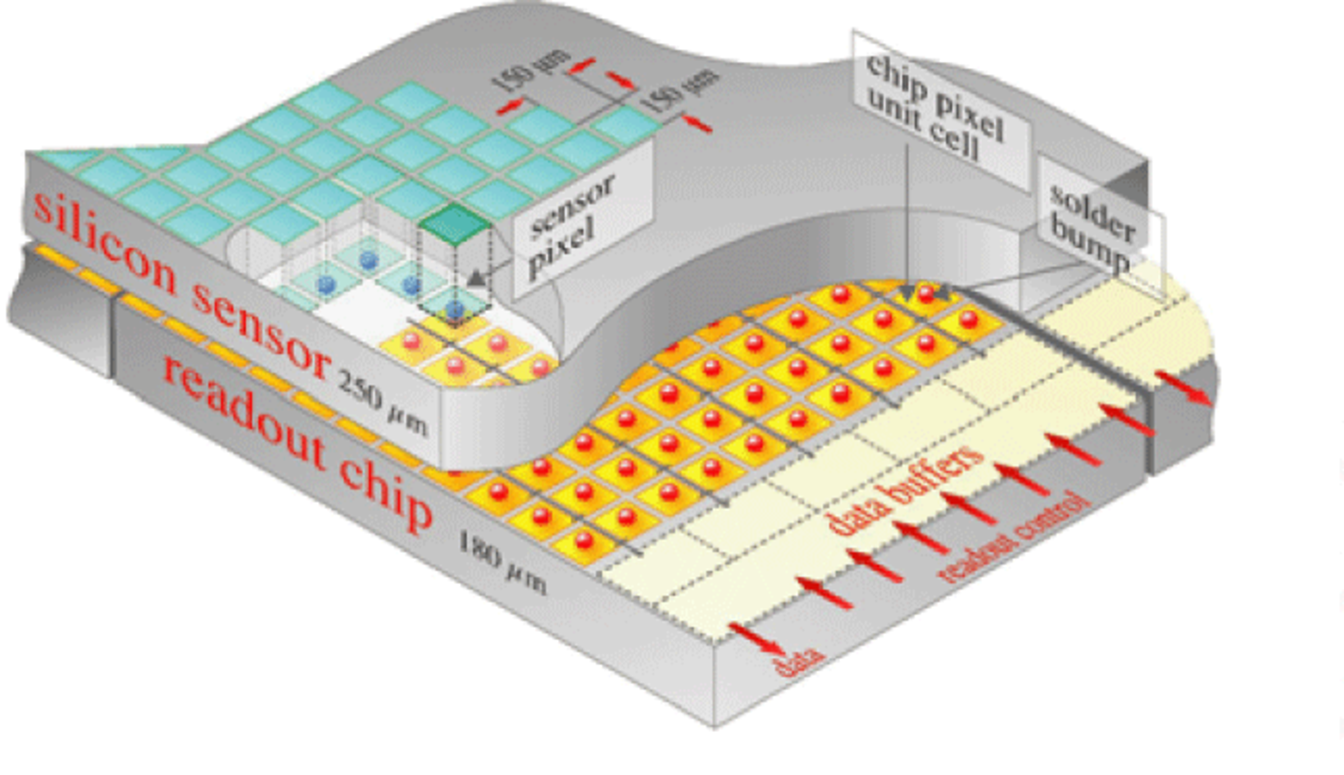
\includegraphics[width=0.8\textwidth]{cms/figs/Pixelement.pdf}
    \caption{
      \label{fig:pixels}
      A diagram showing the pixel component of the tracker subdetector.
    }
  \end{center}
\end{figure}

Immediately outside of the pixel layer is the strip layer.
There are 10 layers of strips through which a charged particle passing through will leave deposits of energy that are read out.
The very large magnetic field in this region from the solenoid is in the same direction as the beam,
and this causes particle trajectories to curve in a direction tangent to the beam direction. 
The radius of this curvature is proportional to the particle's momentum and inversely proportional to the particle's charge according to equation~\ref{eqn:bfieldmomentum}.
Using the hit information from the pixels and strips together,
the momentum of all the charged particles that pass through the tracker is reconstructed and
used as input to the particle flow algorithm~\ref{subs:particleflow} in order to identify particles produced in the collision.
The total material budget of the tracker as a function of radiation and interaction length is shown in figure~\ref{fig:trackerbudget}.
The total depth is seen to be increasing with $|\eta|$ up to where the tracker barrel meets the tracker endcap then decreasing after this point.

\begin{figure}[!htb]
\begin{center}
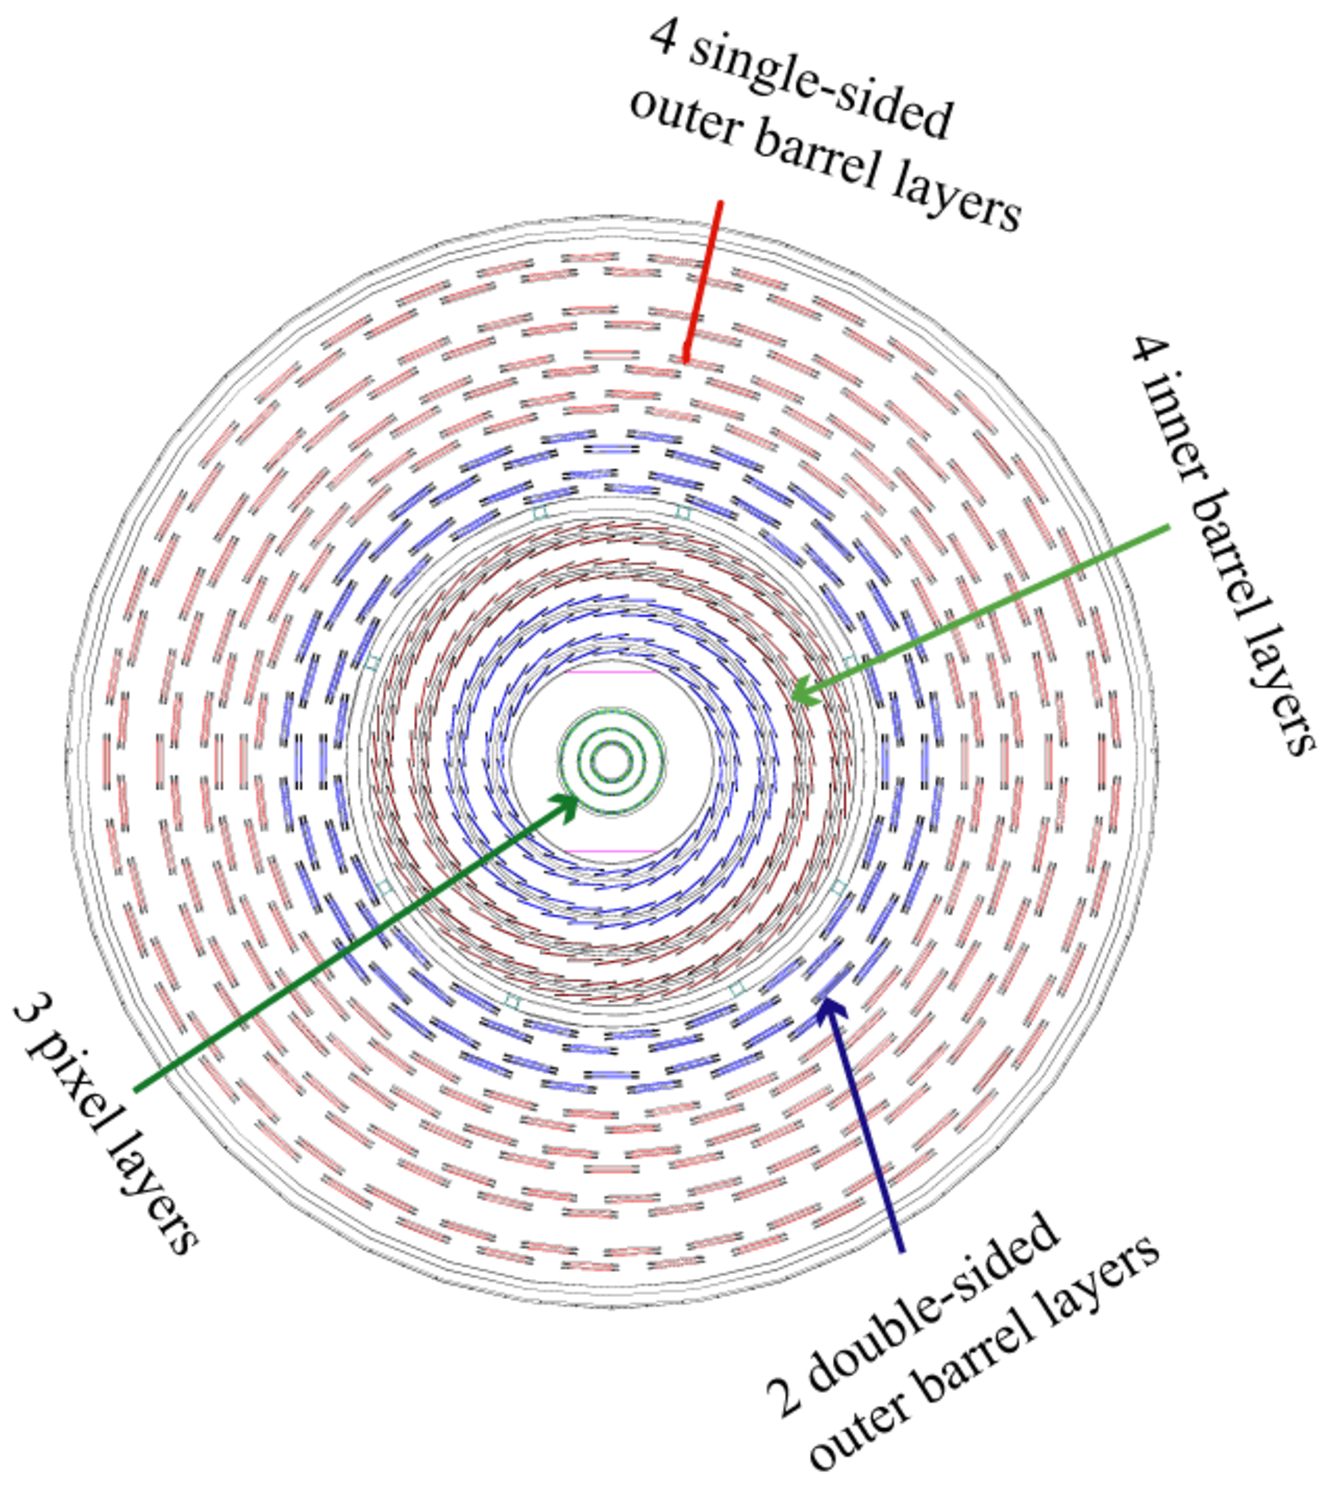
\includegraphics[width=0.8\textwidth]{cms/figs/Barrel.pdf}
\caption{
  A cross-sectional in the x-y plane of the CMS tracking system is shown here.
  The tracker provides excellent coverage for reconstruction of tracks from charged particles for $|\eta| < $2.5.
\label{fig:tracker}
}
\end{center}
\end{figure}

\begin{figure}[!htb]
  \begin{center}
  \begin{tabular}{c c}
    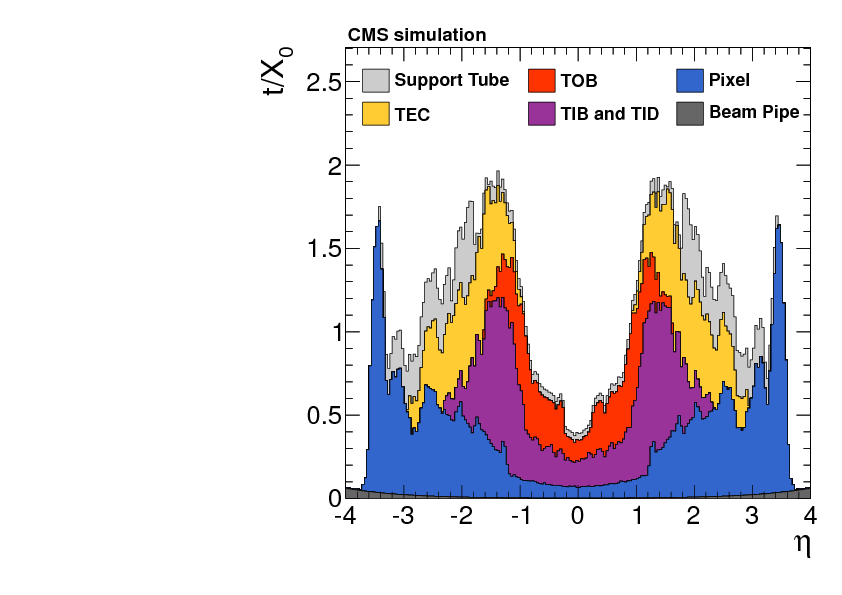
\includegraphics[width=0.4\textwidth]{cms/figs/figs_2011_cmsTracker_MaterialBudget_RadLengths.png} &
    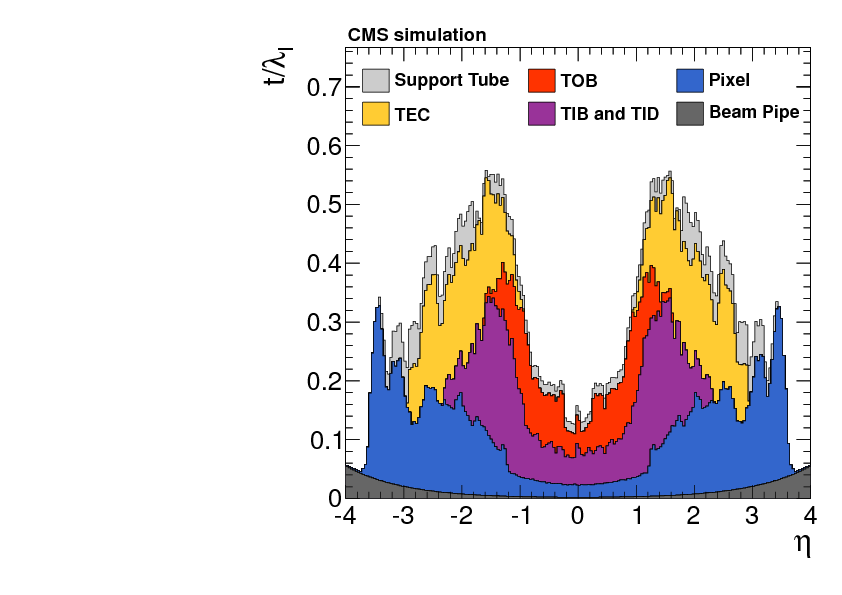
\includegraphics[width=0.4\textwidth]{cms/figs/figs_2011_cmsTracker_MaterialBudget_InteractionLengths.png} \\
  \end{tabular}
    \caption{
      \label{fig:trackerbudget}
      A diagram showing material budget of the tracker as a function of $\eta$ on the x-axis, and radiation lengths (left) and interaction lengths (right).
    }
  \end{center}
\end{figure}


\subsection{Electromagnetic Calorimeter}
\label {subs:ECAL}
The ECAL is split into two regions, the ECAL barrel (EB), and ECAL endcap (EE).
The EB occupies a region in the detector within $|\eta| < 1.479$, and the EE occupies the region with $1.479 < |\eta| < 3.0$.
The geometry can be seen in figure~\ref{fig:ecal_eta}.

\begin{figure}[!htb]
\begin{center}
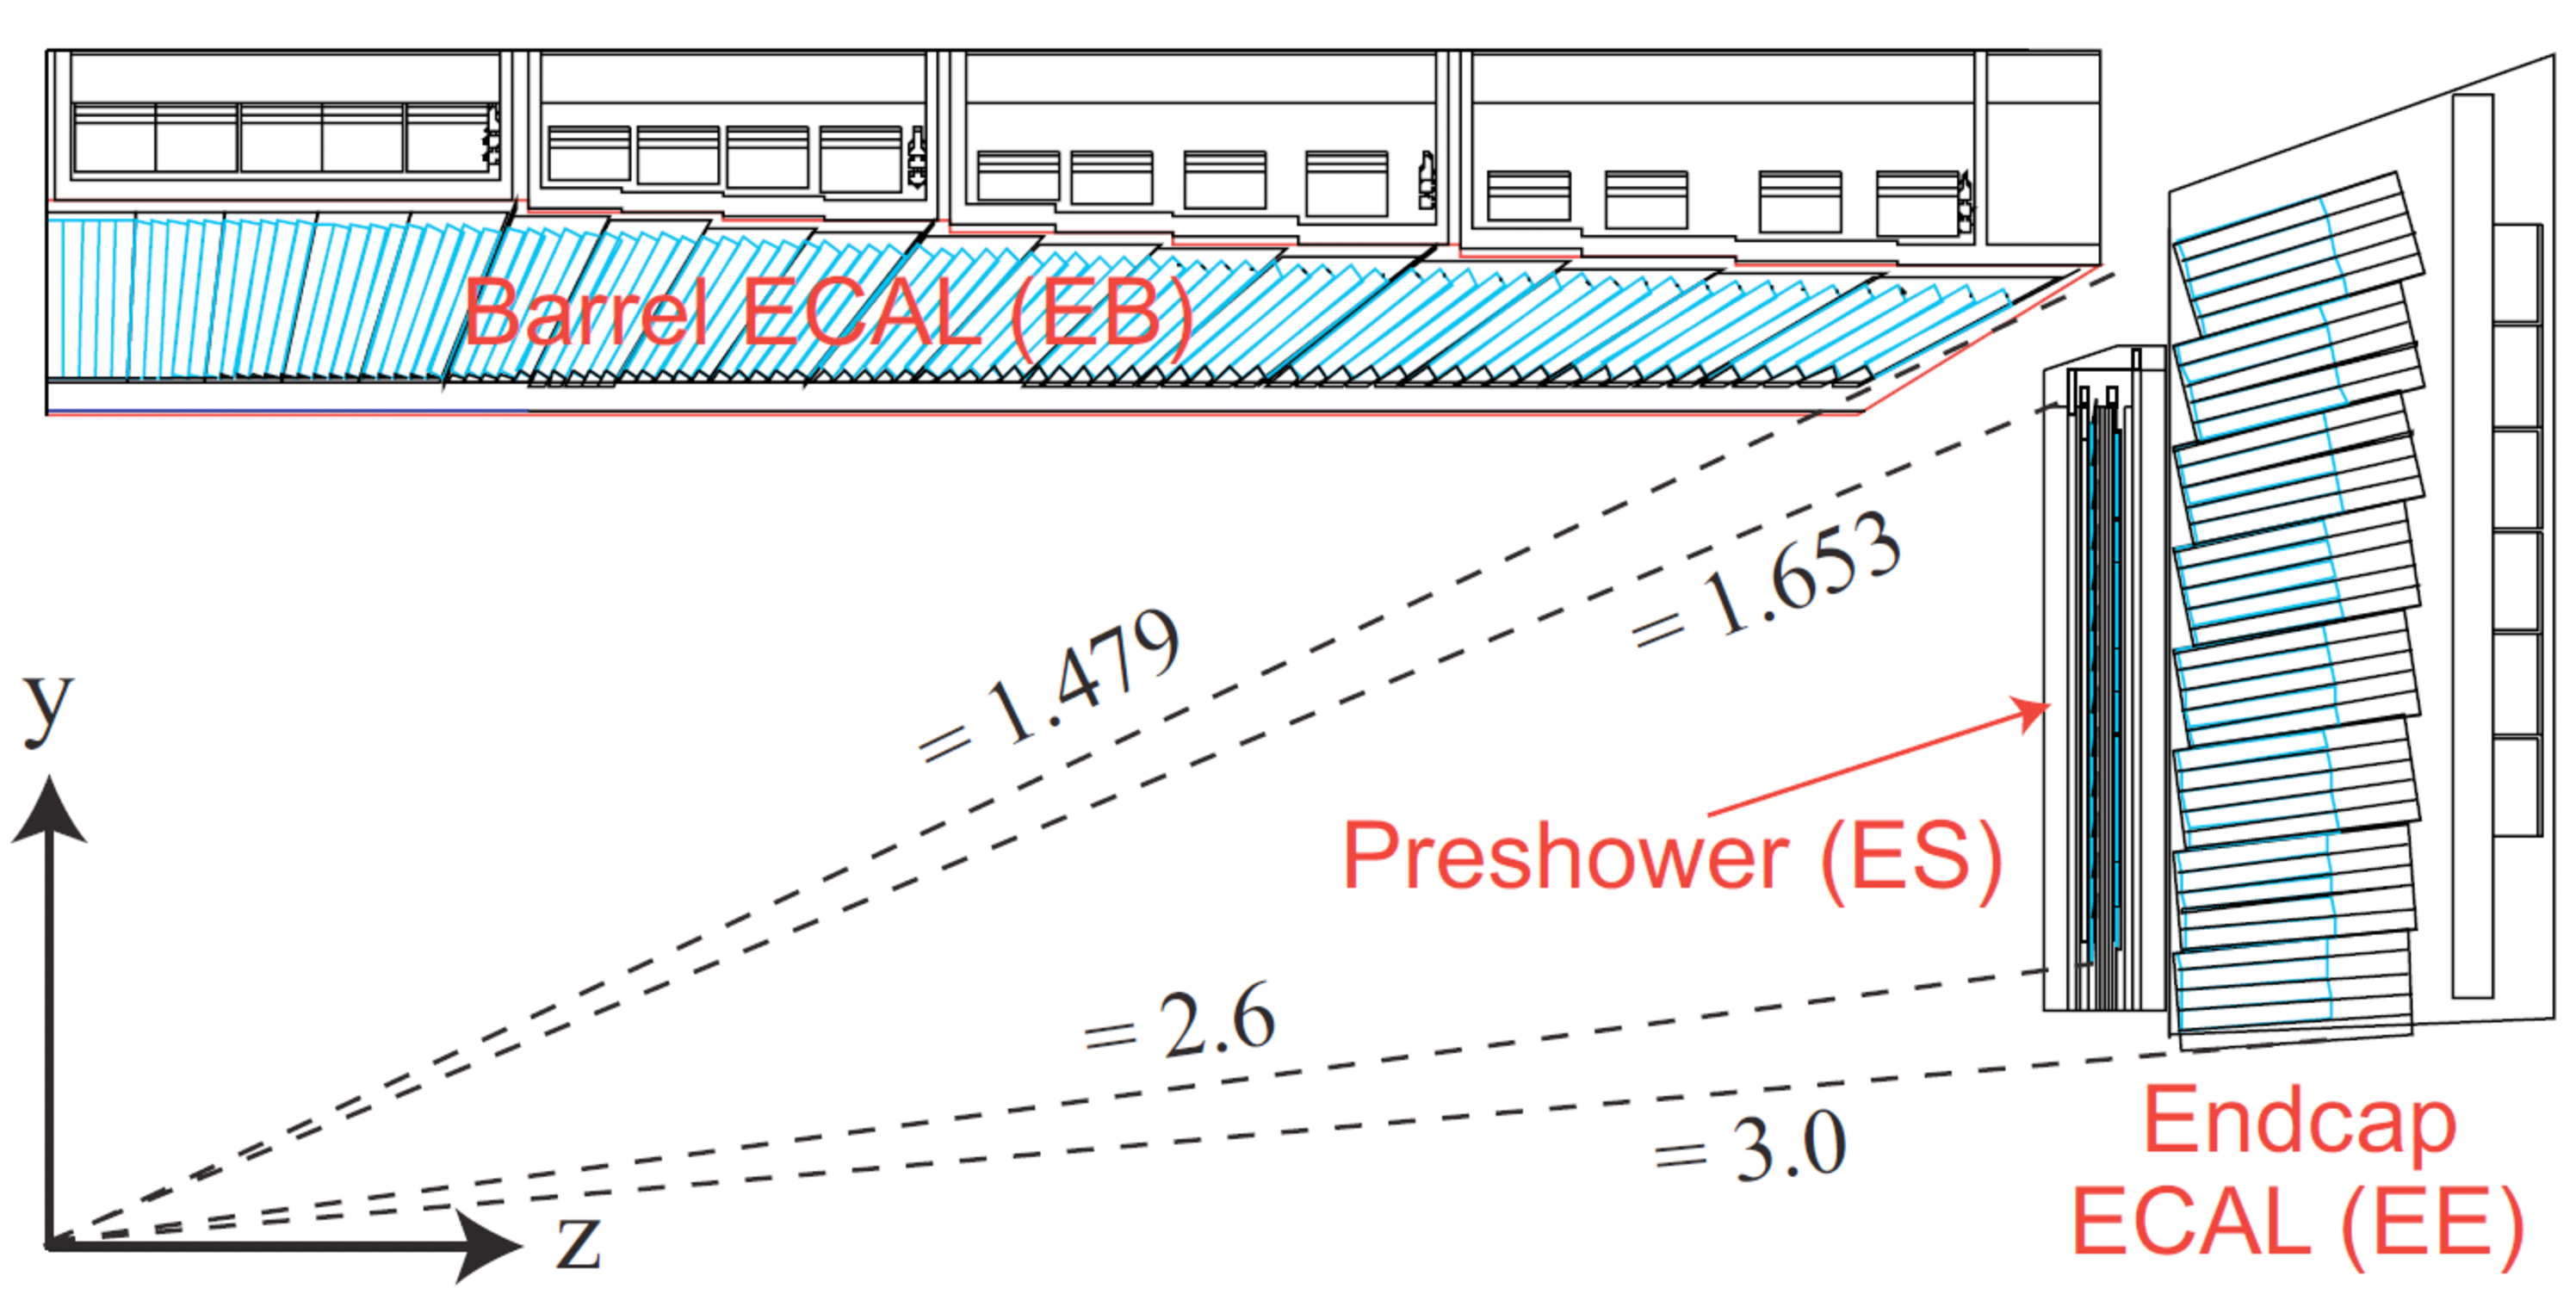
\includegraphics[width=0.8\textwidth]{cms/figs/Figures_Experimental_Apparatus_ECALRapidity.pdf}
\caption{ A cross-sectional view of the CMS ECAL is shown in this figure, with values of $\eta$ shown that determine the coverage of each subdetector.
\label{fig:ecal_eta}
}
\end{center}
\end{figure}

\clearpage

As written previously, the ECAL is made of lead tungstate crystals.
These crystals act as absorbers as well as scintilators.
What this means is that the when electrons or photons are incident on the crystals, they lose energy due to showering.
The showering process can be simply described as a combination of electron-positron pair production, and photon emission.
Leading order diagrams of these processes are shown in figures~\ref{fig:pair_production}~and~\ref{fig:photon_brem}.

\begin{figure}[!ht]
\begin{center}
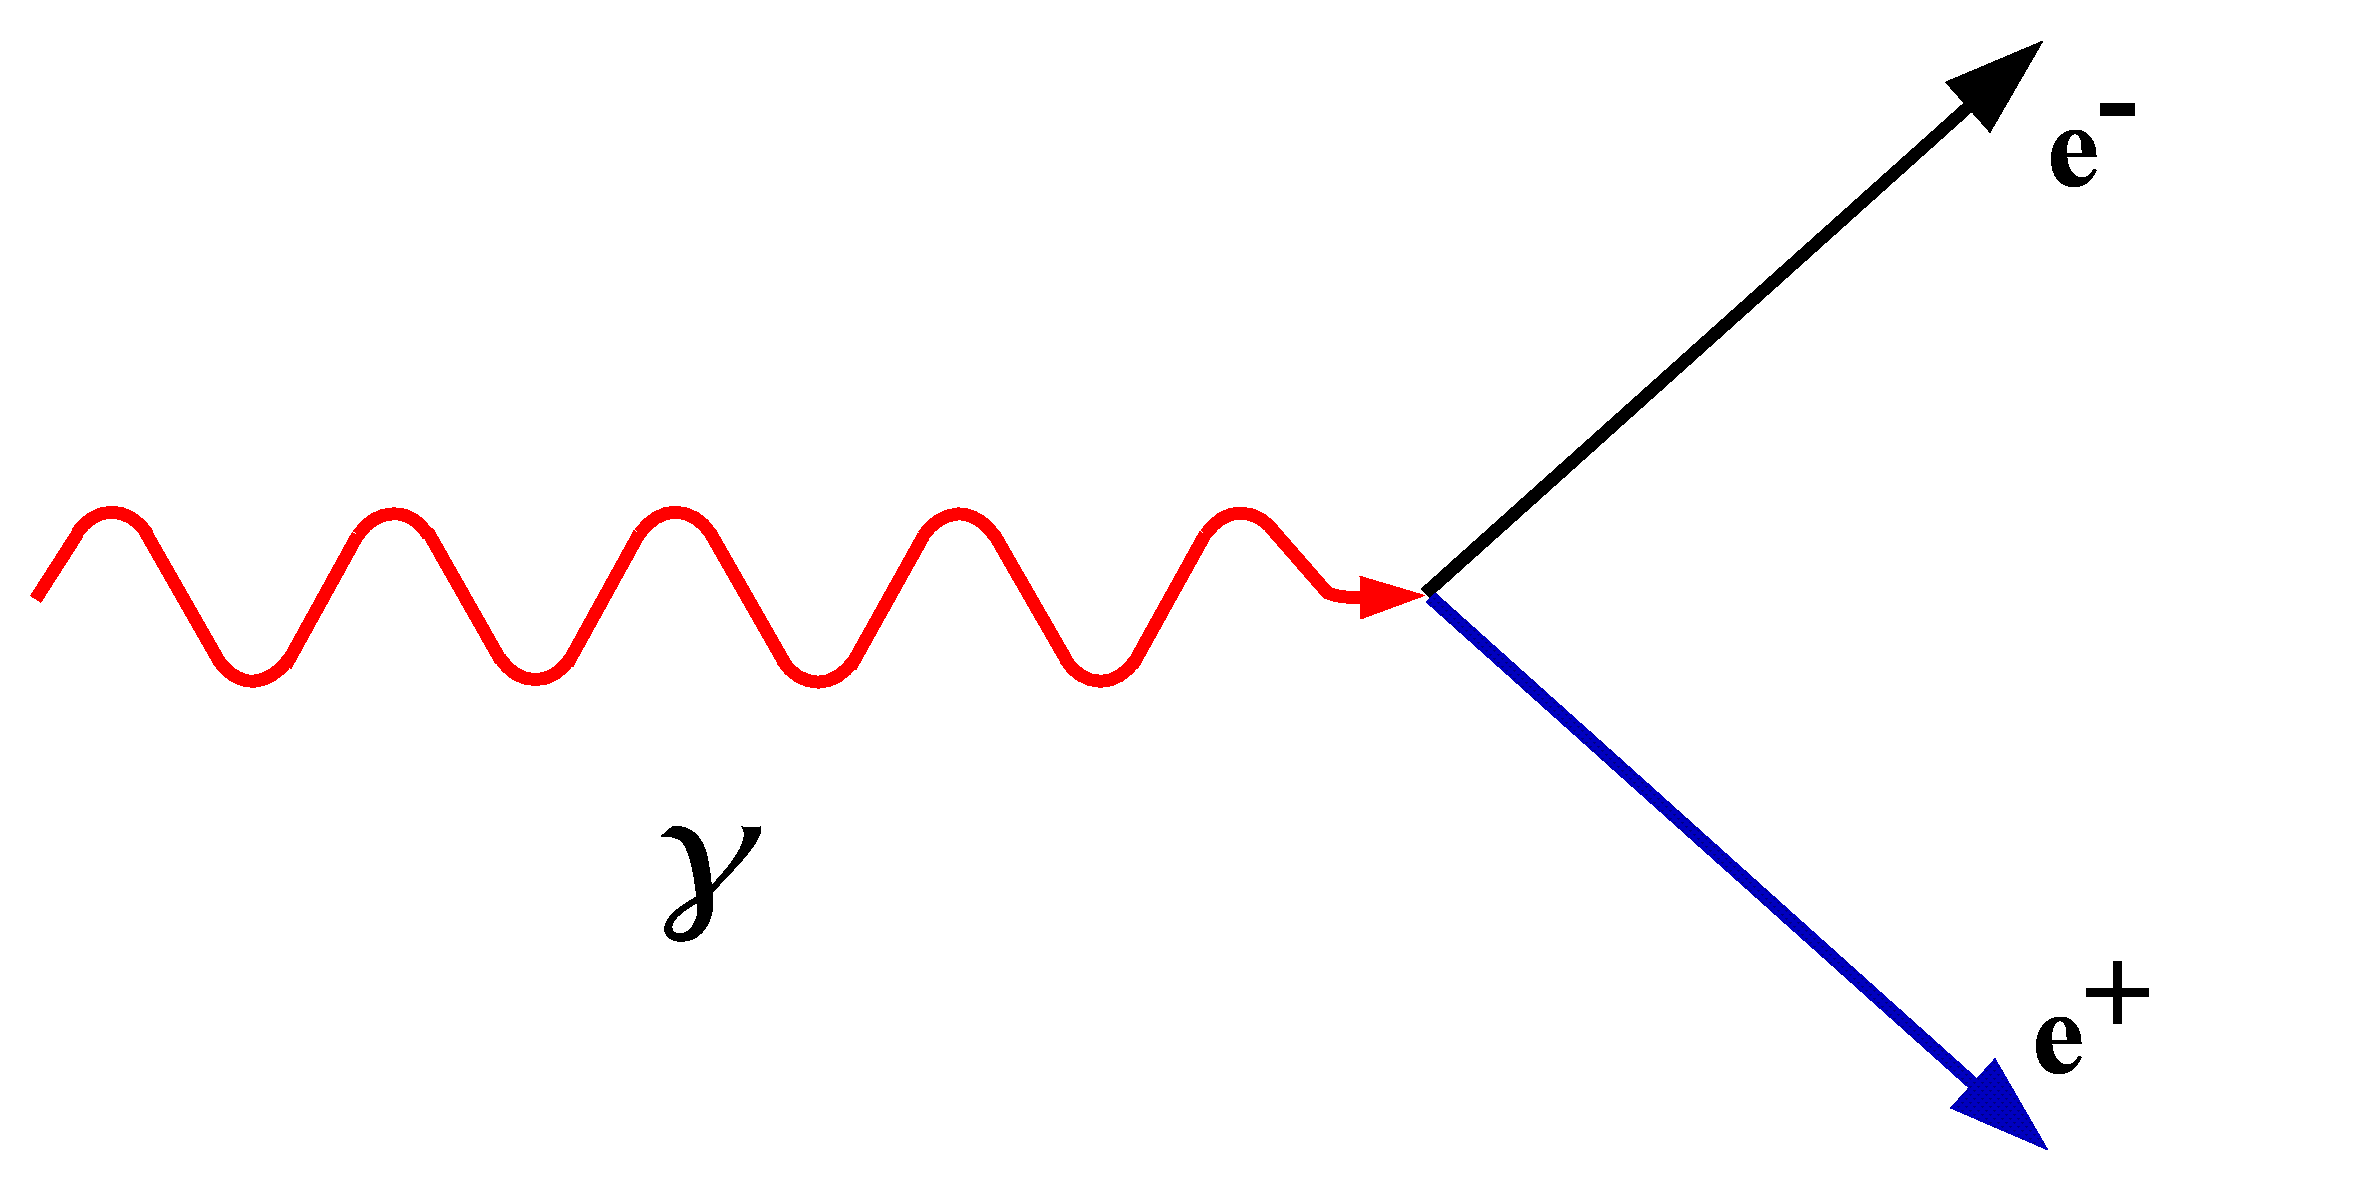
\includegraphics[width=0.8\textwidth]{cms/figs/Pair_Production.png}
\caption{ A feynman diagram is shown depicting electron-positron pair production from a photon initial state.
\label{fig:pair_production}
}
\end{center}
\end{figure}

\begin{figure}[!ht]
\begin{center}
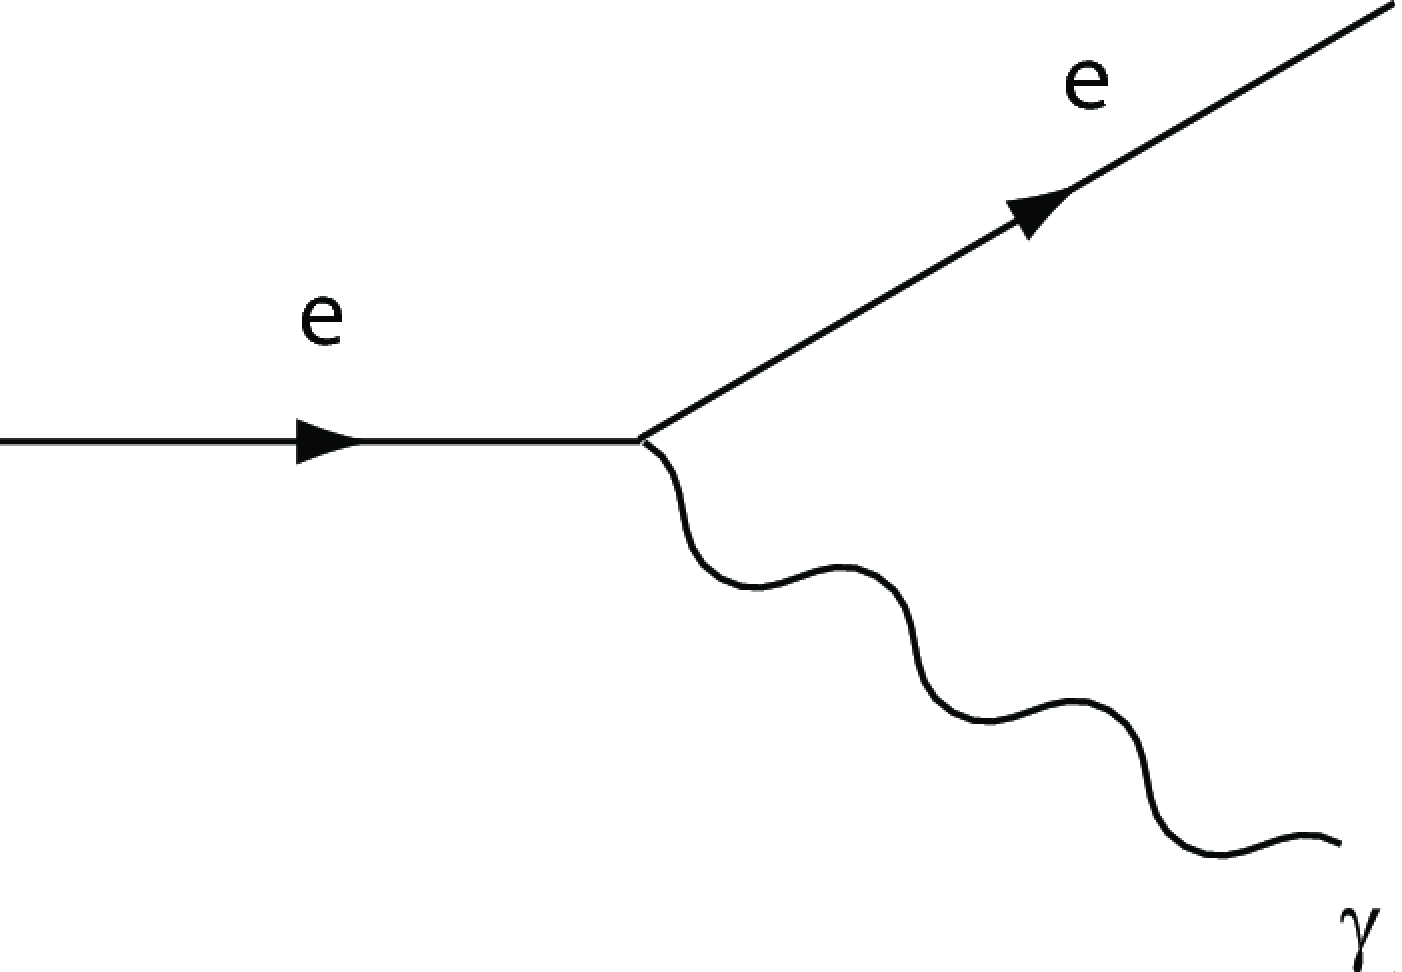
\includegraphics[width=0.8\textwidth]{cms/figs/photon_brem.png}
\caption{
  A feynman diagram is shown of a process where an electron radiates a photon through bremsstrahlung.
\label{fig:photon_brem}
}
\end{center}
\end{figure}

As the initial particle passes through the crystal, it loses energy due to these processes, and this energy is converted to light by the scintilating properties of the crystal.
This light is read out using a avalanche photo-diode (APDs) for each crystal in the EB, and a vacuum phototriode for each crystal in the EE.
The amount of energy absorbed by the crystals can be parameterized by a quantity known as the radiation length ($X_{0}$).
The expected amount of energy left (E(x)) after a particle with initial energy ($E_{0}$)
travels a distance x through an absorbing material is shown in equation~\ref{eqn:radiation_length}.
The CMS ECAL has a depth of \textasciitilde{}25$X_{0}$ at small (0-1.3) and large (1.6-3.0) values of $\eta$.
In between these regions, the depth is larger due to the barrel-like geometry of the ECAL.
Additionally, the ECAL material has a Moli\`ere radius ($\mathrm{R_{M} \simeq 2.19~cm}$) where
$\mathrm{R_{M}}$ is defined as the radius of a cylinder containing on average 90\% of the shower's energy deposition.
Because of the depth and intrinsic resolution, electron and photon energies are measured very well in the ECAL.
There is one exception where the depth of the ECAL is small, and this is where the barrel and endcap meet.
This leads to poor reconstruction of electrons and photons in this region.

\subsection{Hadronic Calorimeter}
\label {subs:HCAL}
The Hadronic Calorimeter (HCAL) is used to measure energies of hadronic particles, such as charged pions, gluons, protons, kaons and neutrons~\cite{hcalperformance}.
It is a sampling calorimeter meaning it has many layers of absorber material (brass) and scintilator material (plastic).
As hadronic particles pass through the HCAL, they interacts with the absorber layers by showering, meaning they decay to multiple lower energy particles.
As these particles shower and the constituents pass through the scintilator, photons are emitted by the scintilating material and then measured by Hybrid-Photo Diodes (HPDs).

When a hadronic particle is incident on the HCAL, a hadronic shower is induced.
Approximately two third of the particles produced in a hadronic shower are charged pions,
and the rest are $\pi_{0}$s which immediately decay to two photons most of the time.
the charged pions in the shower produce scintillating light in the scintilator layer which is measured.
Due to the very large radiation length depth of~\textasciitilde{}5$X_{0}$~per layer of absorber,
the photons produced from the $\pi_{0}$ decays do not leave the absorbing material and as a result are not measured.
The total scintilation light is measured, and the incident particle's energy is inferred from this measurement.
The inferred energy is then subject to fluctuations depending on the relative number of $\pi_{0}$s produced in the shower which are lost in the absorbing layer.

Some detectors however are built to be able to accurately measure the energy lost to electromagnetic effects in the shower, and these are known as ``compensating'' calorimeters.
When a particle is stopped by the HCAL, the energy deposited in all the layers is integrated over a full segment of the HCAL, and used to determine an incident particles energy.
The HCAL at CMS is not able to compensate for these effects, so it must be calibrated offline using particles with a well-known initial energy.

%% The HCAL geometry is such that it is fully contained within the solenoid.
The HCAL is divided into towers, each of which lies behind an integer number of ECAL crystals.
This helps in calibrating the energies of incident particles during reconstruction.
The number of interaction lengths ($\lambda_{int}$) in the HCAL starts at about $\lambda_{int} = 7$ at $\eta = 0$, and increases with eta to the end of the barrel up to $\lambda_{int} = 11$.
There is then a slight decrease in the endcap of $\lambda_{int} = 10$.
The interaction length is used to characterize the longitudinal and transverse profile of hadronic showers.
The expected number of secondary particles produced ($N(x)$)
by a number of particles traveling through the HCAL ($N_{0}$)
is written in equation~\ref{eqn:interaction_length} as a function of $\lambda_{int}$ and the distance traveled (x).

Quarks and gluons produced in proton collisions hadronize to form jets,
and the momentum of these jets can be measured using measurements from both the HCAL and ECAL.

\subsection{Muon System}
\label {subs:MUON}
The muon system is made up of 1400 chambers divided into 3 categories: 610 resistive plate chambers (RPCs), 250 drift tubes (DTs), and 540 cathode strip chambers (CSCs).
It is the only detector subsystem which lies outside of the solenoid, but it is embedded within the return yoke of the solenoid.
Therefore, the magnetic field in the muon system is non-uniform leading to a characteristic s-curve
flight path in the R-$\phi$ plane for muons originating from the center of the detector.
The B-field decreases in the return yoke as the distance from the solenoid increases radially outward leading to the bending radius of the muon decreasing as well.
The information from these systems is used for triggering on events with muons as well as help to identify muons and measure the their properties.
Each system is located in different regions in the detector, with some systems overlapping others.
The DTs cover a region of $|\eta| < 1.2$, the CSCs cover a region of $0.9 < |\eta| < 2.4$, and the RPCs cover a region of $|\eta| < 2.1$.

Each DT is 4 cm wide with a length of wire running all the way down the middle.
A diagram of a DT is shown in figure~\ref{fig:DT}.
The DTs are individually filled with a mixture of Ar and $\mathrm{CO_{2}}$ gas, and when muons pass through the DTs, this gas is ionized.
A voltage difference is maintained between the wire and the outside of the DT such that when the gas is ionized,
the ionized particles drift towards the charged components causing a voltage spike.
The DTs are then arranged in such a way that a muon passing through the region where these are located will leave a hit in multiple DTs.
The muon's trajectory can then be reconstructed using this information.

\begin{figure}[!htb]
  \begin{center}
    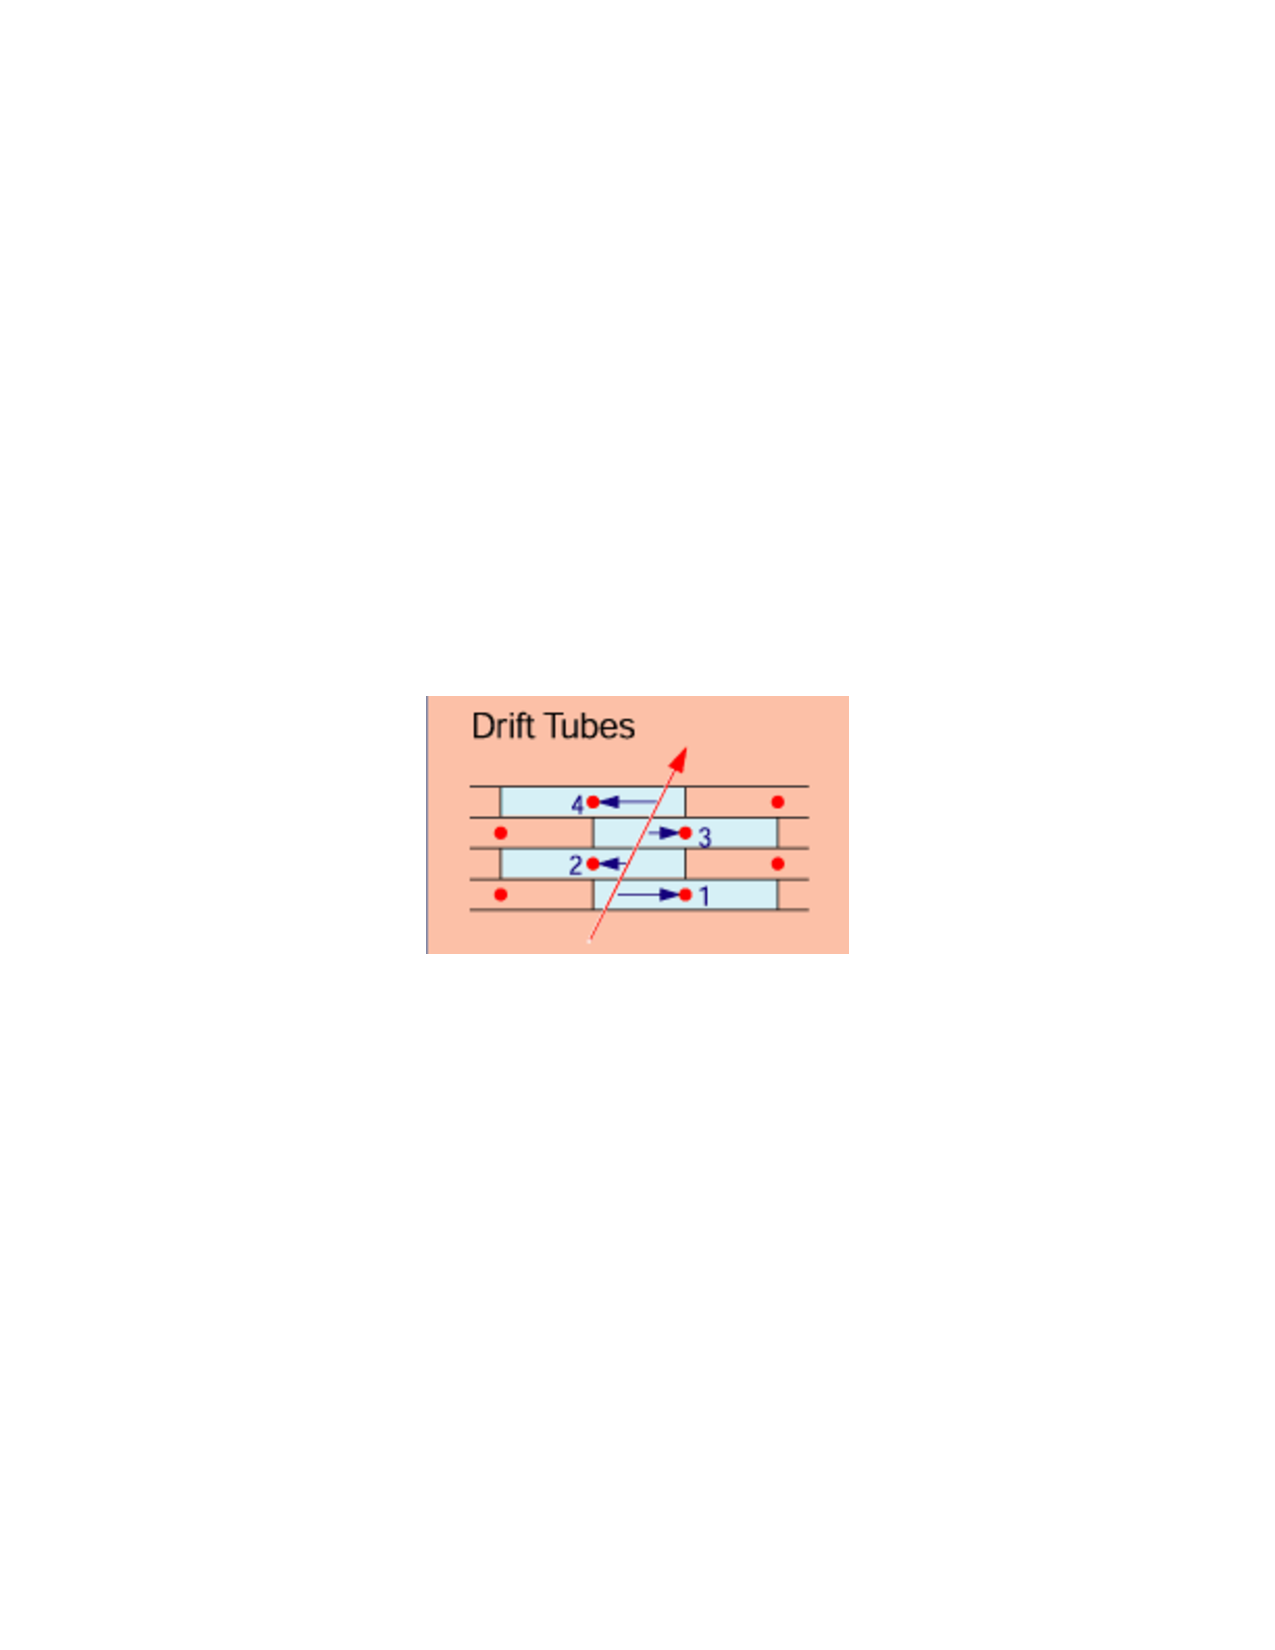
\includegraphics[width=0.8\textwidth]{cms/figs/DT.pdf}
    \caption{
      \label{fig:DT}
      A cartoon depiction of a set of drift tubes is shown in this figure
      where a charged particle passing through the system ionizes the gas,
      and the ions are collected on the wires to detect a signal.      
    }
  \end{center}
\end{figure}

There are 540 CSCs shown in figure~\ref{fig:CSC}.
The CSCs are made up of negatively charged wires (anodes) and positively charged strips (cathodes) within a gas volume.
The gas molecules within this volume are ionized when a muon passes through the volume.
This leads to a measurable hit on both the anodes and cathodes, and they are perpendicular to eachother so that the muon's trajectory can be reconstructed accurately.
There are six layers in each CSC module, which helps to accurately identify muons.

\begin{figure}[!htb]
\begin{center}
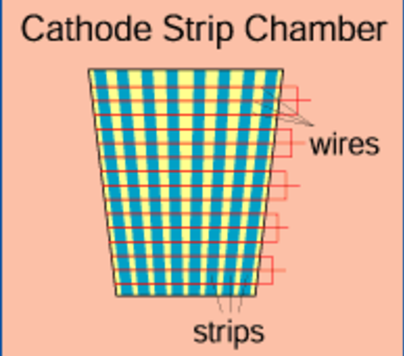
\includegraphics[width=0.8\textwidth]{cms/figs/CSC.pdf}
\caption{ A cartoon depiction of a cathode strip chamber is shown in this figure. 
\label{fig:CSC}
}
\end{center}
\end{figure}

There are 610 resistive plate chambers (RPCs), an example of which is shown in figure~\ref{fig:RPC}.
These are designed to have overlapping trigger coverage with the other components of the muon system for $\eta <$ 2.1.
Each RPC is made of two very high resistance plates, separated by a volume of gas.
They are charged kept at a high voltage and when a muon passes through the gas, electrons are knocked off of the molecules.
Metal strips are used to read out the position of the hit, and the muons momentum is measured with this information.
The readout for the RPCs is very fast (1 ns) which makes it ideal to use for triggering events with good muons.

\begin{figure}[!htb]
  \begin{center}
    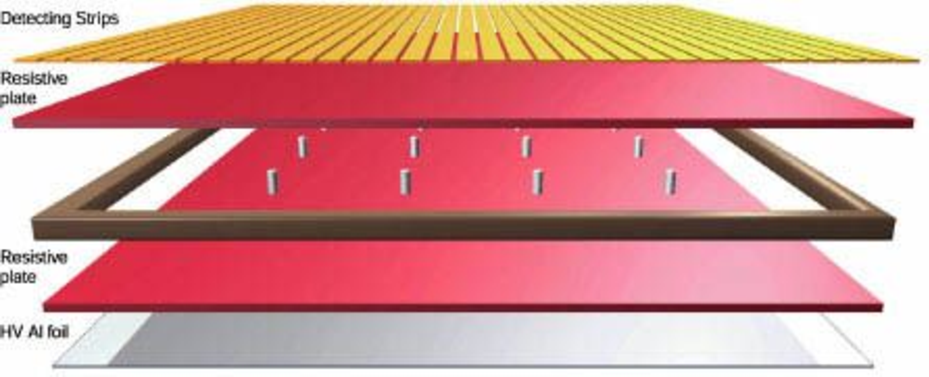
\includegraphics[width=0.8\textwidth]{cms/figs/RPClayers.pdf}
    \caption{
      \label{fig:RPC}
      A cartoon depiction of a resistive plate chamber is shown in this figure. 
    }
  \end{center}
\end{figure}

\section{Physics objects}
The data taken by the CMS detector has to be processed in such a way that all the physics processes that happen in a single collision can be reconstructed.
Each reconstructed collision is called an event.
In each event, there are multiple physics objects that are reconstructed.
The main objects that are pertinent to this analysis are electrons, muons, jets, and photons.
Each of these objects has a unique signature in the detector, but it is still possible for this signature to be faked.
The reconstruction of these objects is discussed in detail in the following sections.

\subsection{Particle Flow}
\label{subs:particleflow}
In order to classify objects, an algorithm named particle flow (PF) is used~\cite{pfReco}. 
The main goal when using the PF algorithm is to account for all energy deposits measured in the detector in a consistent fashion.
The way this is done is by clustering energy deposits measured across all subdetectors into separate PF candidates.
Once an object is classified, the clustering is done again with all the energy associated with the classified object removed.
This process is repeated until all measured energy deposits are accounted for.
For example, a charged hadron would be reconstructed by first identifying a track in the tracker.
Then a check is done to see if this track is consistent with an identified electron, or muon.
If not, all the energy that is associated with this track in the ECAL and HCAL is removed from the event,
and the track measurement is used to describe the particle.
This is done because the precision of measuring charged hadrons is much better in the tracker than in the calorimeters.
This is done iteratively for all particles in the event until there are no tracks left,
then all that remain are the neutral energy deposits.
The use of particle flow leads to greatly improved measurements of jets since more of the jet energy is measured using the tracker.
This also leads to a higher precision measurement of missing transverse energy for the same reasons.

The objects that are identified by this algorithm are listed below.
In order to further reduce fakes from contaminating our signal region, we make additional cuts to help classify objects.
These cuts are described in detail in the following section for each object we are interested in.

\begin{itemize}
\item muon          
\item photon        
\item charged hadron
\item neutral hadron
\item electron      
\end{itemize}

\subsection{Vertex Determination and Pileup}
\label{ssec:vtxandpileup}
The LHC collides protons in large bunches to maximize the probability of a hard collision.
Multiple pairs of protons interact at each bunch crossing,
and the number of interactions is stochastic but depends on the beam intensity.
Each proton proton collision can produce particles that get reconstructed,
and when these particles are reconstructed they are associated to a specific proton proton collision using charged particle information.
It is important to identify which proton-pair interaction is responsible for triggering the event being studied.
Every particle track is associated with a unique vertex,
and the primary vertex is chosen by finding the vertex with the largest sum of $\mathrm{(p_{T})^{2}}$ of tracks associated with that vertex.
Neutral candidates do not have associated tracks, so they are defined to always be from the primary vertex.
The energy of objects affected by this reassociation is recalibrated, and this calibration is described in section~\ref{ssec:jets}.

Pileup is defined as energy in the detector which does not come from the primary collision or primary interaction.
There are two primary sources of pileup, in-time pileup (ITPU), and out-of-time pileup (OOTPU).
ITPU occurs when protons other than those in the primary interaction interact in the same bunch crossing,
and the particles produced are reconstructed.
OOTPU occurs mainly due to the fact that protons are collided with a frequency of 25ns,
and the timing resolution of some detector components is not fast enough to resolve which bunch crossing certain reconstructed particles came from.
The number of expected pileup events can be determined using equation~\ref{eqn:pileup} where$\mathcal{L}_{inst.}$ is the instantaneous luminosity,
$\sigma(p-p)_{inelastic}$ is the total inelastic scattering cross section for protons,
and $f_{collision}$ is the collision frequency.
For 2015, this value is 12.75.

\begin{equation}
\label{eqn:pileup}
  \mathrm{N_{pileup} = \mathcal{L}_{inst.}*\sigma(p-p)_{inelastic}*f_{collision}}
\end{equation}

All of the energy from pileup comes from proton-proton interactions other than the primary interaction.
These ``soft'' interactions produce predominantly hadronic final states,
and the majority of these interactions are due to gluons scattering off of quarks or other gluons.
These final states inherently do not have \MET\ due to particles escaping detection due to them being hadronic,
and this leads to a balance in the overall energy deposited in the detector.
There are still contributions to \MET\ from to pileup due to the poor resolution of jets in CMS.
A calibration is applied to account for pileup according to the method described in section~\ref{sec:t1met}.


\subsection{Isolation}
\label{ssec:isolation_summary}
Isolation is a concept that is very important when identifying leptons, and photons.
Isolation can be simply described as the total energy in the detector near an object of interest.
When leptons or photons from the primary interaction are not produced together with colored objects,
they are deemed prompt.
Non-prompt leptons, such as those from a b-quark decaying semi-leptonically,
and non-prompt photons such as those from $\pi ^{0}$ decay,
are always produced in conjunction with a hadronic shower.
These non-prompt objects are then very likely to be non-isolated due to the hadronic energy nearby.
The distance between two objects ($\Delta$R) is defined by equation~\ref{eqn:DR},
where $\phi$ is the angle measured in plane transverse to the beam direction,
and $\eta$ is the psuedorapidity defined by equation~\ref{eqn:psuedorapidity}.
In the equation for $\eta$, the variable $\theta$ is defined as the angle measured from the beam axis to the axis of the transverse plane to the beam axis.
In particle physics, $\eta$ is preferred over $\theta$ when describing a particle's momentum along the beam axis because changes in $\eta$ are lorentz invariant,
whereas the same is not true for changes in $\theta$.

\begin{equation}
  \label{eqn:DR}
  \Delta R = \sqrt{\Delta\eta^{2}+\Delta\phi^{2}}
\end{equation}

\begin{equation}
  \label{eqn:psuedorapidity}
  \eta = -\ln(\mathrm{tan}(\frac{\theta}{2}))
\end{equation}

The choice of what to include when calculating isolation is defined differently for each object and will be described in the following sections.

\subsection{leptons and photons}
\label{ssec:lepsandphots}
Z bosons decay leptonically to $e\bar{e}$, $\mu\bar{\mu}$, and $\tau\bar{\tau}$~pairs 3.363 $\pm$ 0.004\%, 3.366 $\pm$ 0.007\%\ and 3.370 $\pm$ 0.008\% of the time respectively.
The rest of the time they decay to neutrinos, or to quark-antiquark pairs.
This analysis focuses on decays to $e\bar{e}$ and $\mu\bar{\mu}$.
This is due to the fact that $\tau$s have a large mass and short lifetime which leads to them decaying.
This is further complicated by the fact that $\tau$s decay to an electron ($\mu$) and two neutrinos 17.85 $\pm$ 0.05\% (17.36 $\pm$ 0.05\%) of the time,
and the rest of the time the $\tau$ decays to hadronic final state particles.
This leads to worse measurements in leptonic final states due to the missing energy from not detecting the neutrinos,
and makes it hard to distinguish $\tau$s from jets in hadronic channels.
In order to keep the analysis simple, this search is done in final states with $Z\rightarrow ee$ and $Z\rightarrow\mu\bar{\mu}$ only,
and when referencing leptons, only electrons and muons are considered.
It is also important to be able to identify photons in order to measure one of the main backgrounds.

The depth of the ECAL is \textasciitilde{}25 radiation lengths which means electrons and photons lose almost all of their energy in the ECAL.
Another thing that helps to distinguish electrons from photons is that electrons will deposit energy in the silicon tracker whereas photons will not.
Therefore, a track can be matched to energy deposits in the ECAL to help identify electrons.
Similarly, a track found to correspond to a hit in the ECAL can be used to help determined that the energy deposited in the ECAL was not from a photon.

A different approach is taken to identify and measure muons in the CMS detector.
Since muons are charged, they leave hits in the silicon detector which can be reconstructed as a track.
The ECAL and HCAL are designed to contain all measureable energy,
but due to the minimum ionizing nature of muons, muons are able to pass through these subdetectors without depositing much energy.
The muon subdetector is the outermost layer of the CMS detector, and it is designed to identify muons.
Muon tracks can be measured independently in the muon subdetector,
and the measurement is matched to a set of hits in the tracker to determine the final muon energy.

The main thing all of these objects have in common is they are produced in interactions that do not have a hadronic component.
Quantifying this energy is done by calculating the particles isolation, as described in section~\ref{ssec:isolation_summary},
and is used to discriminate against unwanted physics processes.



\subsection{jets}
\label{ssec:jets}
A jet is an object used to represent a single parton, and it can be simply described as a substantial amount of hadronic activity concentrated in a single region of the detector.
The region is defined using the ``anti-$\mathrm{k_{T}}$'' (ak) algorithm~\cite{antikt} with a jet radius of 0.4.
For jets in this analysis, the charged candidates not associated with the primary vertex are removed before clustering. 
This removes some unwanted energy from pileup, and the jets are then calibrated in order to more accurately reflect the energy of the particles they represent.

The jet energy corrections are done in multiple levels, labeled as L1,L2 and L3.
A detailed procedure of how the corrections are applied can be found here~\cite{CMS-DP-2015-044}.
Jets are corrected such that the calibrated energy is as close as possible to the parton that produced the jet.
The corrections are derived using MC, and each level corrects for different effects in the following way:
L1 corrects for pileup,
L2 corrects for different responses in the detector as a function of $\eta$,
and L3 corrects the overall energy scale.
The L1 correction is done by assuming a flat overall energy density from pileup in the detector which is calculated per event,
and then subtracting this energy from the jet using the jet area to determine the overall energy contributed from pileup.
The L2 correction is done by selecting di-jet events where one of the jets is central($\eta < 0.8$) and the second jet is non-central ($\eta > 0.8$).
Scale factors are then derived to correct the energy measurement for the non-central jet in separate regions of $\eta$.
The L3 correction is done by deriving scale factors as a function of jet \pt\ which correct the jet energy to match the true energy of the parton that the jet came from.

In addition to the L1, L2 and L3 corrections, residual corrections are derived in data control regions to correct for differences in the detector response to jets between data and MC.
This is done in a region with at least one photon or a Z boson which decays to two leptons, where the boson recoils off of a jet.
The photon and leptons are measured with better resolution than the jets, so scale factors are derived as a function of \pt\ to correct the detector response of jets.
The full description of cuts used to define jets for the analysis is defined in sub-section~\ref{ssec:jetsel}.

This is to acknowledge all the other members of the CMS experiment who made it possible to produce
the figures and tables appearing in this chapter.
